\usetikzlibrary{arrows.meta}
\tikzset{%
  >={Latex[width=2mm,length=2mm]},
  % Specifications for style of nodes:
            minerbase/.style = {rectangle,
                           minimum width=3cm, minimum height=1cm,
                           text centered, font=\sffamily},
            base/.style = {rectangle, rounded corners, draw=black,
                           minimum width=3cm, minimum height=1cm,
                           text centered, font=\sffamily},
  censoredminer/.style = {minerbase, draw=red!30},
  uncensoredminer/.style = {minerbase, draw=blue!30},
  majority/.style = {base, fill=blue!30},
  minority/.style = {base, fill=red!30},
    common/.style = {base, fill=green!30},
 blacklist/.style = {base, minimum width=2cm, fill=orange!70}
}

\subsection{Expected Results}
Suppose we have client $C$, a censored miner, sitting behind a censorship firewall, a client $U$ who is uncensored, and a block $B_0$ which is the last valid block known by all parties before the partition emerged. Now suppose $U$ mines block $B_1$ containing a transaction with a blacklisted keyword. U transmits an \textit{inv} message about $B_1$. Since $C$ has never seen $B_1$, it requests the full block from $U$ by transmitting a \textit{getdata} message for $B_1$. $U$ begins transmitting $C$ a \textit{block} message for $B_1$, but the censorship firewall notices a blacklisted keyword and intervenes. This can be seen in Figure~\ref{fig:censor}.
Regardless as to whether the censorship firewall truncates the transmission of $B_1$ from $U$ to $C$ or simply resets the connection, the end result is that $C$ will never receive $B_1$ but will know of its existence (since it received the \textit{inv} message about $B_1$).

To better understand what would happen if a node knew about the existence of a block which it could never retrieve, we examined the source code to \texttt{bitcoind}. In Bitcoin, clients learn of new blocks by listening for block header broadcasts. Once it hears of a new block header, the client attempts to download the block. The reference client keeps track of the active chain; however, it will only ever update the active chain once the block header and the full block are both received and validated. According to a comment in the source\footnote{Specifically, line 2668 of \texttt{validation.cpp} in \texttt{bitcoind} version 0.14~\cite{bitcoind-source}}, this logic was introduced to defend against malicious miners trying to obtain a competitive advantage by broadcasting headers but withholding blocks. Therefore, we expect $C$ to continue mining off $B_0$, the previously known block, thereby causing a fork.

\begin{figure}[h]
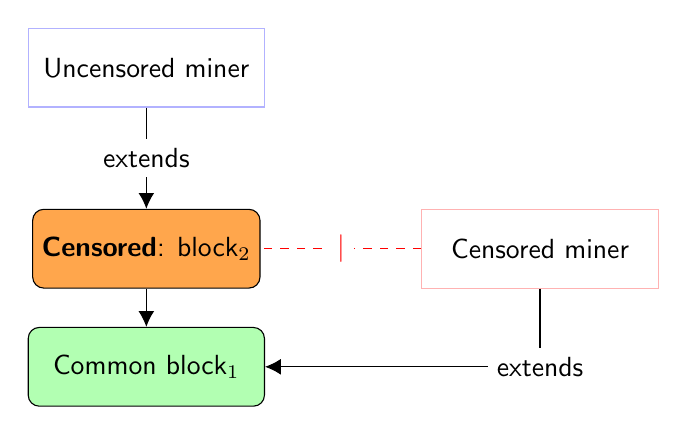
\begin{tikzpicture}[every node/.style={node distance=1.5cm,fill=white, font=\sffamily}, align=center]
  %\node (majority2)[majority, above of=majority1] {Majority block};
  \node (bad)   [blacklist]                {\textbf{Censored}: block$_2$};

  \node (fmine)[uncensoredminer, above of=bad, yshift=.8cm] {Uncensored miner};
  \node (cmine)[censoredminer, right of=bad, xshift=3.5cm] {Censored miner};
  \node (start)  [common, below of=bad]    {Common block$_1$};

    \draw[->]             (bad) -- (start);
    \draw[->]             (fmine) -- node{extends} (bad);
    \draw[->]             (cmine) |- node{extends} (start);
    \draw[red,dashed]             (cmine) --node{$|$} (bad);
\end{tikzpicture}
\caption{After a censored block is mined, miners try extending different blocks}
\label{fig:censor}
\end{figure}

\subsubsection{Censored minority}
Figure~\ref{fig:censored-minority} shows the scenario in which the minority of hash power is behind the censor. Censored miners will see future blocks added by uncensored miners, but will not be able to validate their chain, so they will be ignored.

\begin{figure}[h]
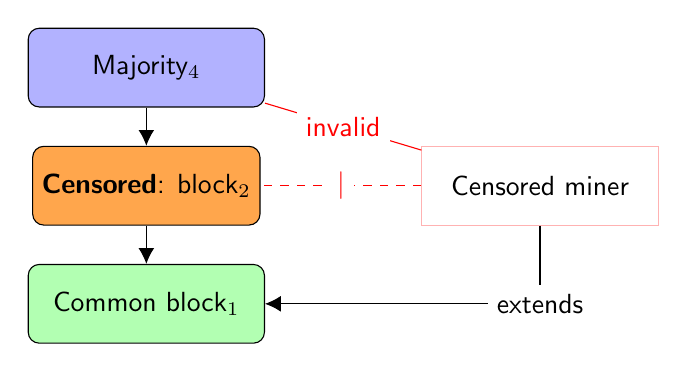
\begin{tikzpicture}[every node/.style={node distance=1.5cm,fill=white, font=\sffamily}, align=center]
  %\node (majority2)[majority, above of=majority1] {Majority block};

  \node (bad)   [blacklist]                {\textbf{Censored}: block$_2$};
  \node (start)  [common, below of=bad]    {Common block$_1$};
  \node (majority1)[majority, above of=bad] {Majority$_4$};
  \node (miner)[censoredminer, right of=bad, xshift=3.5cm] {Censored miner};

    \draw[red]          (miner) -- node{invalid} (majority1);
    \draw[red,dashed]     (miner) -- node{$|$} (bad);
    \draw[->]             (miner) |- node{extends} (start);
    \draw[->]             (majority1) -- (bad);
    \draw[->]             (bad) -- (start);
\end{tikzpicture}
\caption{A model in which the minority of hash power is located behind the censor}
\label{fig:censored-minority}
\end{figure}

\subsubsection{Censored majority}
If censored miners mine faster than uncensored miners, the two forks will eventually grow to be of equal length. Censored miners will only be able to see one of the forked paths while uncensored miners will be able to see (and mine off of) both. This can be seen in Figures~\ref{fig:censored-majority} and~\ref{fig:censored-majority2}.


\begin{figure}[h]
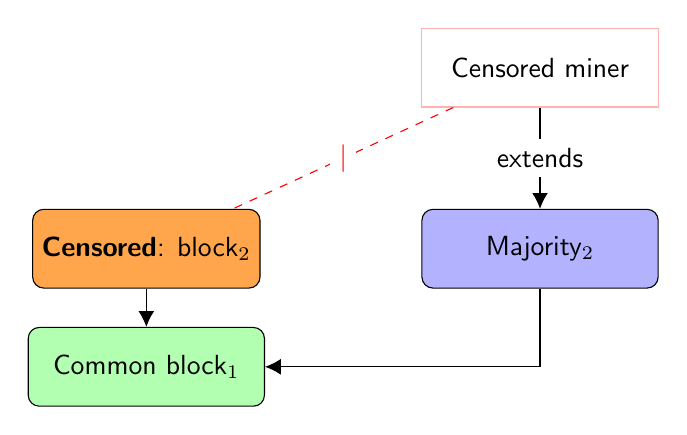
\begin{tikzpicture}[every node/.style={node distance=1.5cm,fill=white, font=\sffamily}, align=center]
  %\node (majority2)[majority, above of=majority1] {Majority block};

  \node (bad)   [blacklist]                {\textbf{Censored}: block$_2$};
  \node (start)  [common, below of=bad]    {Common block$_1$};
  \node (majority1)[majority, right of=bad, xshift=3.5cm] {Majority$_2$};
  \node (miner)[censoredminer, above of=majority1, yshift=.8cm] {Censored miner};

    \draw[->]          (miner) -- node{extends} (majority1);
    \draw[red,dashed]     (miner) -- node{$|$} (bad);
    \draw[->]             (majority1) |- (start);
    \draw[->]             (bad) -- (start);
\end{tikzpicture}
\caption{A model in which the majority of hash power is located behind the censor}
\label{fig:censored-majority}
\end{figure}

\begin{figure}[h]
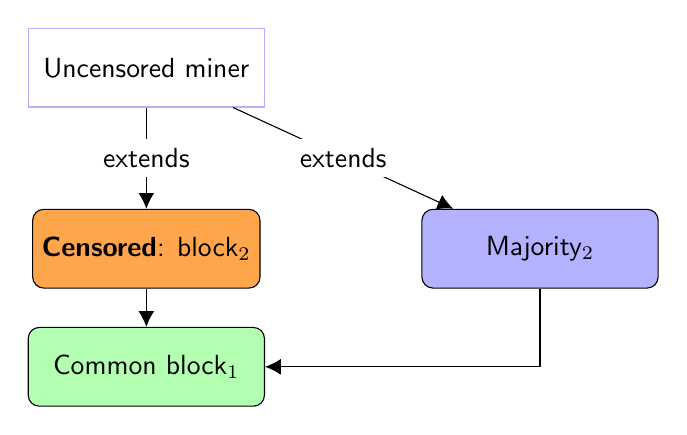
\begin{tikzpicture}[every node/.style={node distance=1.5cm,fill=white, font=\sffamily}, align=center]
  %\node (majority2)[majority, above of=majority1] {Majority block};

  \node (bad)   [blacklist]                {\textbf{Censored}: block$_2$};
  \node (start)  [common, below of=bad]    {Common block$_1$};
  \node (majority1)[majority, right of=bad, xshift=3.5cm] {Majority$_2$};
  \node (miner)[uncensoredminer, above of=bad, yshift=.8cm] {Uncensored miner};

    \draw[->]          (miner) -- node{extends} (majority1);
    \draw[->]     (miner) -- node{extends} (bad);
    \draw[->]             (majority1) |- (start);
    \draw[->]             (bad) -- (start);
\end{tikzpicture}
\caption{Uncensored miners can mine off of either block when the forked chains are of equal length}
\label{fig:censored-majority2}
\end{figure}

In this scenario, one fork can be mined off of by all nodes while the other can only be mined off of by uncensored nodes. Therefore, the first fork is likely to grow more quickly than the second, meaning that it will become accepted as the main chain. This will prevent transactions containing censored keywords from ever being accepted into the main chain (Figure~\ref{fig:censored-majority3}).

\begin{figure}[h]
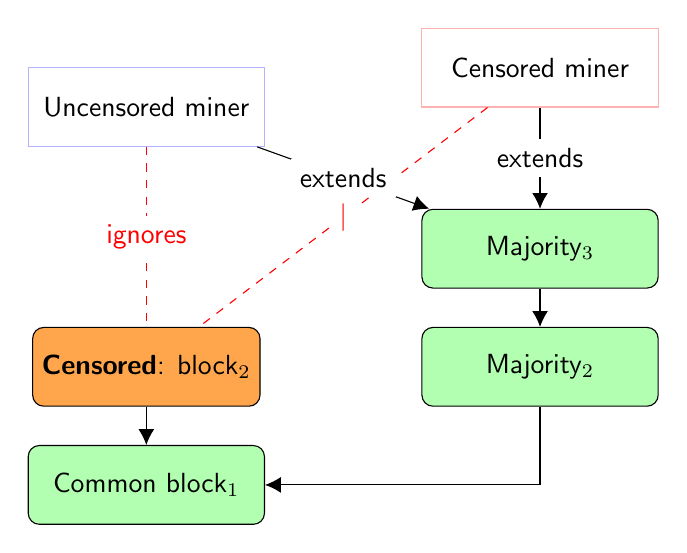
\begin{tikzpicture}[every node/.style={node distance=1.5cm,fill=white, font=\sffamily}, align=center]
  %\node (majority2)[majority, above of=majority1] {Majority block};

  \node (bad)   [blacklist]                {\textbf{Censored}: block$_2$};
  \node (start)  [common, below of=bad]    {Common block$_1$};
  \node (majority1)[common, right of=bad, xshift=3.5cm] {Majority$_2$};
  \node (majority2)[common, above of=majority1] {Majority$_3$};
  \node (cminer)[censoredminer, above of=majority2, yshift=.8cm] {Censored miner};
  \node (fminer)[uncensoredminer, above of=bad, yshift=1.8cm] {Uncensored miner};

    \draw[red,dashed]     (cminer) -- node{$|$} (bad);
    \draw[red,dashed]     (fminer) -- node{ignores} (bad);
    \draw[->]     (cminer) --node{extends} (majority2);
    \draw[->]     (fminer) --node{extends} (majority2);
    \draw[->]             (majority1) |- (start);
    \draw[->]             (bad) -- (start);
    \draw[->]             (majority2) -- (majority1);
\end{tikzpicture}
\caption{Since the majority of mining power is mining off one fork, that fork will eventually grow to be longer than the other and all miners will agree on it}
\label{fig:censored-majority3}
\end{figure}
